\documentclass[12pt]{article}
\usepackage{blindtext}
\usepackage[a4paper, total={170mm, 220mm}]{geometry}
\usepackage[table]{xcolor}
\usepackage{graphicx}
\usepackage{amsmath}
\usepackage{imakeidx}
\usepackage{float}
\usepackage{pdfpages}
\usepackage[spanish]{babel}
\usepackage[affil-it]{authblk}
\renewcommand{\familydefault}{\sfdefault}

\makeindex[columns=3, title=Alphabetical Index, intoc]

%·······································································································

\usepackage{hyperref}
\hypersetup{
    colorlinks=true,
    linkcolor=blue,
    filecolor=magenta,      
    urlcolor=blue,
    }

\urlstyle{same}

%·······································································································

%·······································································································


\makeindex[columns=3, title=Alphabetical Index, intoc]


\graphicspath{{images/}} %configuring the graphicx package
%Gummi|065|=)
\usepackage{tcolorbox}
\tcbuselibrary{listingsutf8} % o listings o minted


\usepackage{rotating}

%·······································································································



\title{\textbf{INFORME DE PROYECTO} \\ \textbf{CONTROL DE VELOCIDAD DE AUTO}}



\author{Alumno: Patricio Germán Silva\thanks{Correo electrónico: \texttt{silvap@fcal.uner.edu.ar}} \\ Profesor: Germán Hatchmann\thanks{Correo electrónico: \texttt{hachmanng@fcal.uner.edu.ar}}}
\affil{\textbf{Introducción a VHDL}  \\ \textbf{Ingeniería en Mecatrónica}}

\begin{document}
\maketitle

%·······································································································


\thispagestyle{empty}
\newpage
\tableofcontents
\thispagestyle{empty}
\newpage
\pagenumbering{arabic}



%·······································································································

\section{Introducción}

Se realizará el diseño, descripción en VHDL y simulación de un sistema capaz de realizar el control de un auto bimotor seguidor de linea. El diseño debe contemplar:
\begin{itemize}
\item Control de dirección y velocidad para un driver L293D.
\item Control de un display de siete segmentos donde se muestra información de velocidad y modo de funcionamiento.
\item Comunicación mediante interfaz UART y protocolo rs232 (TTL) con una velocidad de 9600 baudios, 8 bits, de datos, 1 bit de stop, sin paridad, sin control de flujo. Solo se requiere recepción.
\item Para la comunicación se agrega una capa de protocolo, de frame de ancho fijo, compuesto por un byte de header, un byte de comando, dos bytes de datos y un byte de tráiler, sin suma de comprobación.
\end{itemize}

Para el desarrollo se utiliza el software \textbf{Xilinx Vivado 2024.1}. Por ultimo, se comprobará el correcto funcionamiento del desarrollo en una placa \textbf{DIGILENT Artix-7 FPGA modelo Arty A7-100T (xc7a100tcsg324-1)}. 

\begin{figure}[H]
    \centering
    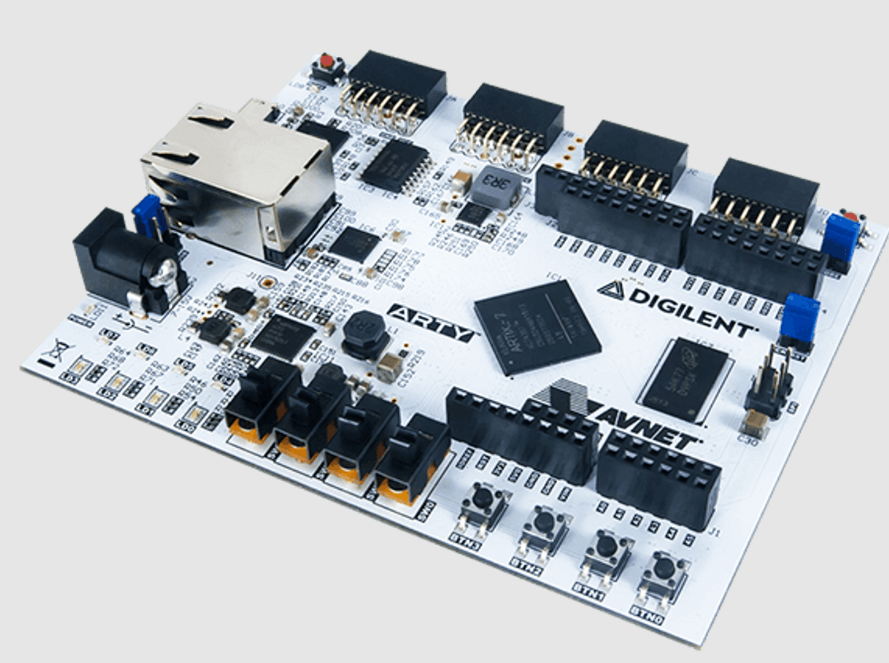
\includegraphics[width=0.6\textwidth]{digilent-arty}
    \caption{DIGILENT  Artix-7 FPGA modelo Arty A7-100T}
\end{figure}

\newpage


Los comandos son los siguientes:
\\

    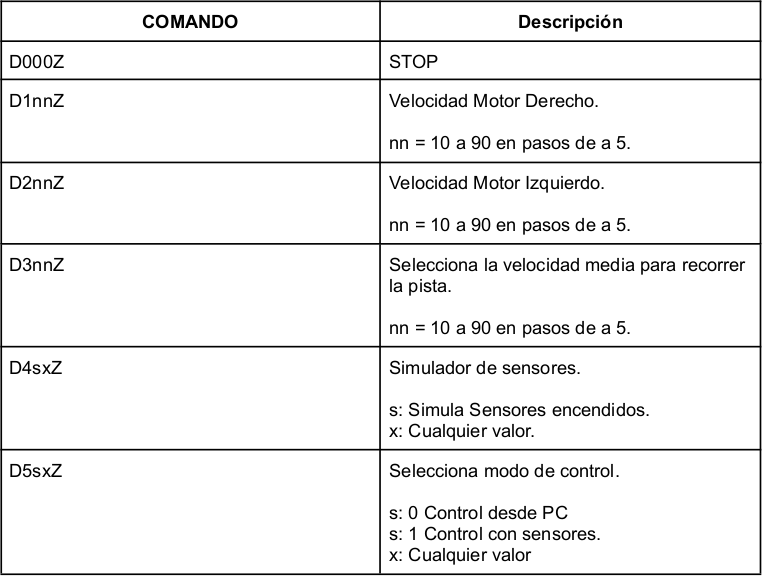
\includegraphics[width=0.8\textwidth]{det-protocolo}



\newpage

%·······································································································
\section{Diseño de la solución}

El diseño se lleva a cabo en diferentes módulos específicos para cada tarea, que serán los siguientes:
\begin{itemize}
\item UaRx: modulo Uart RX para la recepción desde la PC
\item UaTx: modulo Uart TX, cuya única finalidad es hacer echo de la información recibida por UaRx.
\item CommProtRx: modulo que valida un paquete del protocolo de comunicación, e incorpora una detección de timeout.
\item DecodeCmd: Interpreta los comandos recibidos.
\item HBridgeCtrl: recibe una dirección y velocidad y genera una salida PWM según los parámetros establecidos.
\item ToDisplay: Envia información a un display de 7 segmentos con punto decimal
\item Módulos auxiliares: módulos contadores, generadores de baud rate y PWM y decodificadores de 7 segmentos.
\end{itemize}

\subsection{Puertos de I/O}

{\rowcolors{2}{}{gray!20}
\begin{tabular}{|p{2.5cm}|p{2.5cm}|p{1.3cm}|p{1.8cm}|p{7.5cm}|}
\hline			
\textbf{NOMBRE} & \textbf{DIRECCION} & \textbf{PIN}	& \textbf{HEADER} & \textbf{DESCRIPCION} \\
\hline
piIMClk &
IN &
E3 &
- &
Clock de sistema 100MHz
\\

piIMEna &
IN &
A8 &
SW0 &
Enable
\\

piIMRst &
IN &
C11 &
SW1 &
Reset
\\

piIMRx &
IN &
A9 &
- &
Salida al puerto TX del PC
\\

piIMSensors[0] &
IN &
B8 &
BTN0 &
Simula sensor externo izquierdo
\\

piIMSensors[1] &
IN &
B9 &
BTN1 &
Simula sensor interno izquierdo
\\

piIMSensors[2] &
IN &
C9 &
BTN2 &
Simula sensor interno derecho
\\

piIMSensors[3] &
IN &
D9 &
BTN3 &
Simula sensor externo derecho
\\

poIMDirMD[0] &
OUT &
J5 &
LED4 &
Dir1 – Segun L243D
\\

poIMDirMD[1] &
OUT &
H5 &
LED5 &

\\

poIMDirMI[0] &
OUT &
T10 &
LED6 &
Dir2 – Segun L243D
\\

poIMDirMI[1] &
OUT &
T9 &
LED7 &

\\

poIMDot &
OUT &
U11 &
IO26 &
Punto decimal del display de 7 segmentos
\\

poIMPowerMD &
OUT &
N17 &
IO40 &
Salida PWM derecho – 100Hz
\\

poIMPowerMI &
OUT &
P18 &
IO41 &
Salida PWM izquierdo – 100Hz
\\

poIMSevSeg[0] &
OUT &
V16 &
IO33 &
Display – Segmento A
\\

poIMSevSeg[1] &
OUT &
M13 &
IO32 &
Display – Segmento B
\\

poIMSevSeg[2] &
OUT &
R10 &
IO31 &
Display – Segmento C
\\

poIMSevSeg[3] &
OUT &
R11 &
IO30 &
Display – Segmento D
\\

poIMSevSeg[4] &
OUT &
R13 &
IO29 &
Display – Segmento E
\\

poIMSevSeg[5] &
OUT &
R15 &
IO28 &
Display – Segmento F
\\

poIMSevSeg[6] &
OUT &
P15 &
IO27 &
Display – Segmento G
\\

poIMStat &
OUT &
G6 &
LED0\_R &
200ms blink en cada comando valido
\\

poIMTx &
OUT &
D10 &
- &
Salida al puerto RX del PC
\\

\hline
\end{tabular}}


\subsection{Esquemático general}
Todos los módulos son instanciados e interconectados dentro del bloque principal IMain, el diseño general es el siguiente:
\begin{figure}[H]
    \centering 
	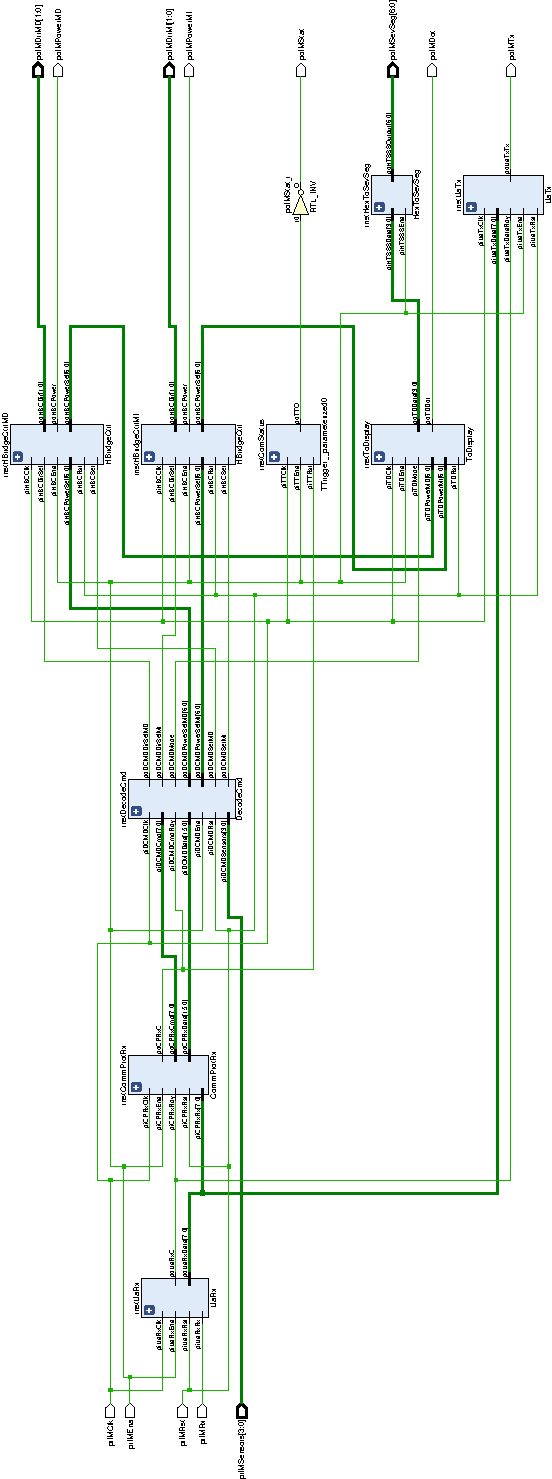
\includegraphics{Integrador-crop}
\end{figure}

\section{Módulos}
A continuación se describen los módulos desarrollados
\subsection{UaRx}
Formado por una maquina de estado y un generador de baudrate. El puerto RX conectado al UART recibe desde la PC paquetes de datos de 8 bits a 9600 baudios, sin control de paridad ni control de flujo, con 1 bit de stop, totalizando un PDU de 10 bytes. Cuando un nuevo dato se recibe se genera un pulso de 1 clock de duración que notifica el evento.

\begin{figure}[H]
    \centering
    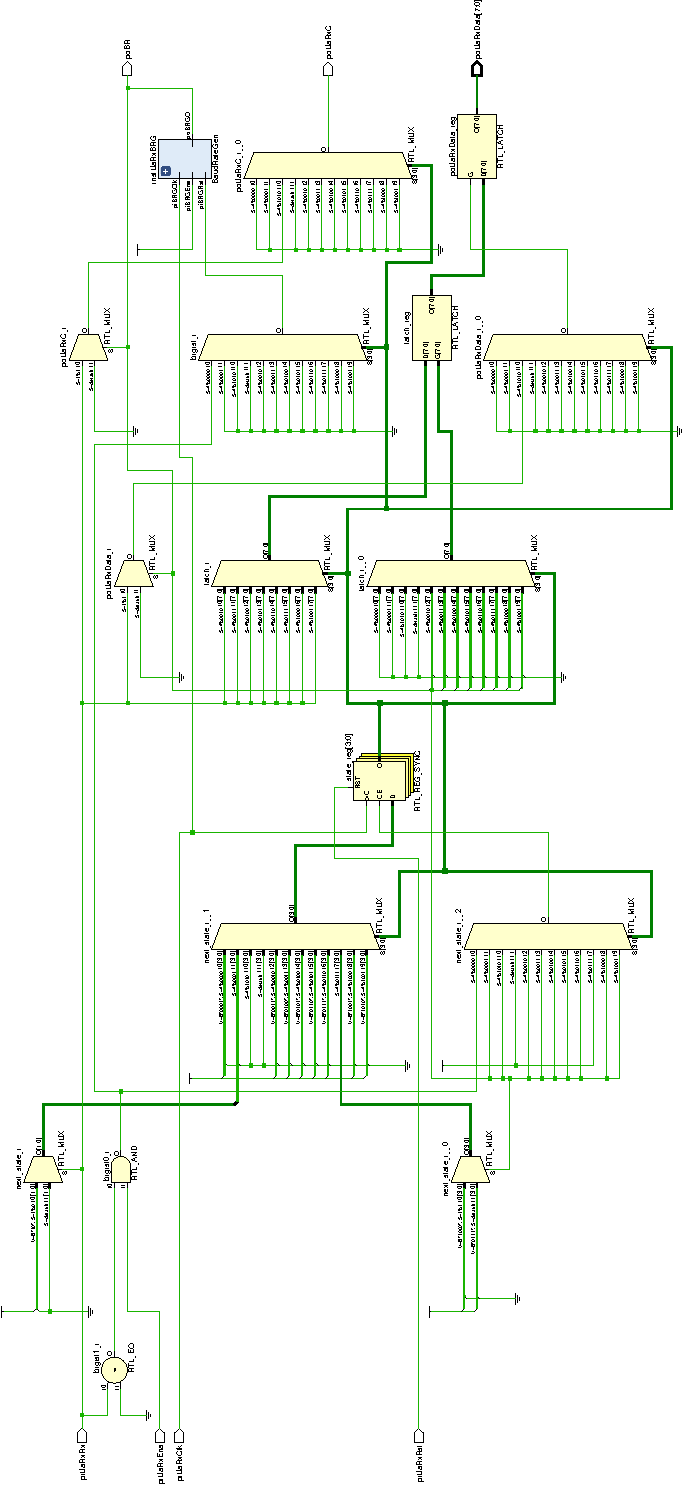
\includegraphics[angle=270, width=\textwidth]{uart-rx-crop}
    \caption{Esquemático del módulo \textbf{UaRx}}
\end{figure}

El diseño contempla un error de baudrate del 3.5\%, y la recepción de un nuevo bit de start de hasta un 45\% antes de finalizar el periodo de bit stop del PDU anterior.

El generador de baudrate genera, tras un reset, un primer pulso de un periodo \textbf{T/2}

\subsection{UaTx}
Formado por una maquina de estado y un generador de baudrate. El puerto TX conectado al UART envía a la PC paquetes de datos con la misma especificación que el modulo UaRx. El envio de un nuevo paquete de datos se inicia mediante un pulso en el puerto piUaTxDataReady, cuando se finaliza el envio el modulo notifica con un pulso de un clock de duración-

\begin{figure}[H]
    \centering
    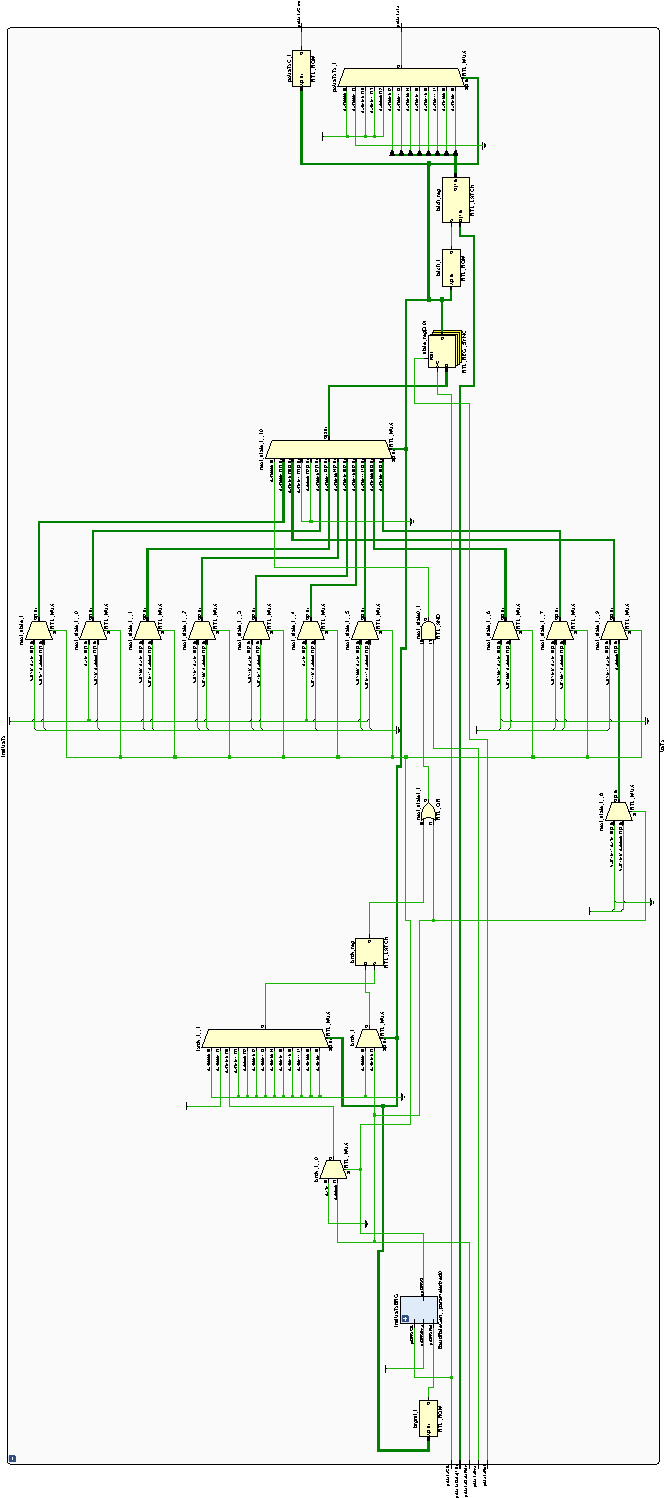
\includegraphics[angle=270, width=\textwidth]{uart-tx-crop}
    \caption{Esquemático del módulo \textbf{UaTx}}
\end{figure}

El diseño contempla iniciar el envío de un nuevo paquete de datos durante el envio del bit de stop del PDU anterior.

\subsection{CommProtRx}
Formado por una maquina de estado y un temporizador de tipo TTrigger, por cada PDU RX recibido analiza si conforma un paquete de protocolo válido, y genera un pulso de clock, poniendo el byte de comando y los dos bytes de datos en el bus de salida.

\begin{figure}[H]
    \centering
    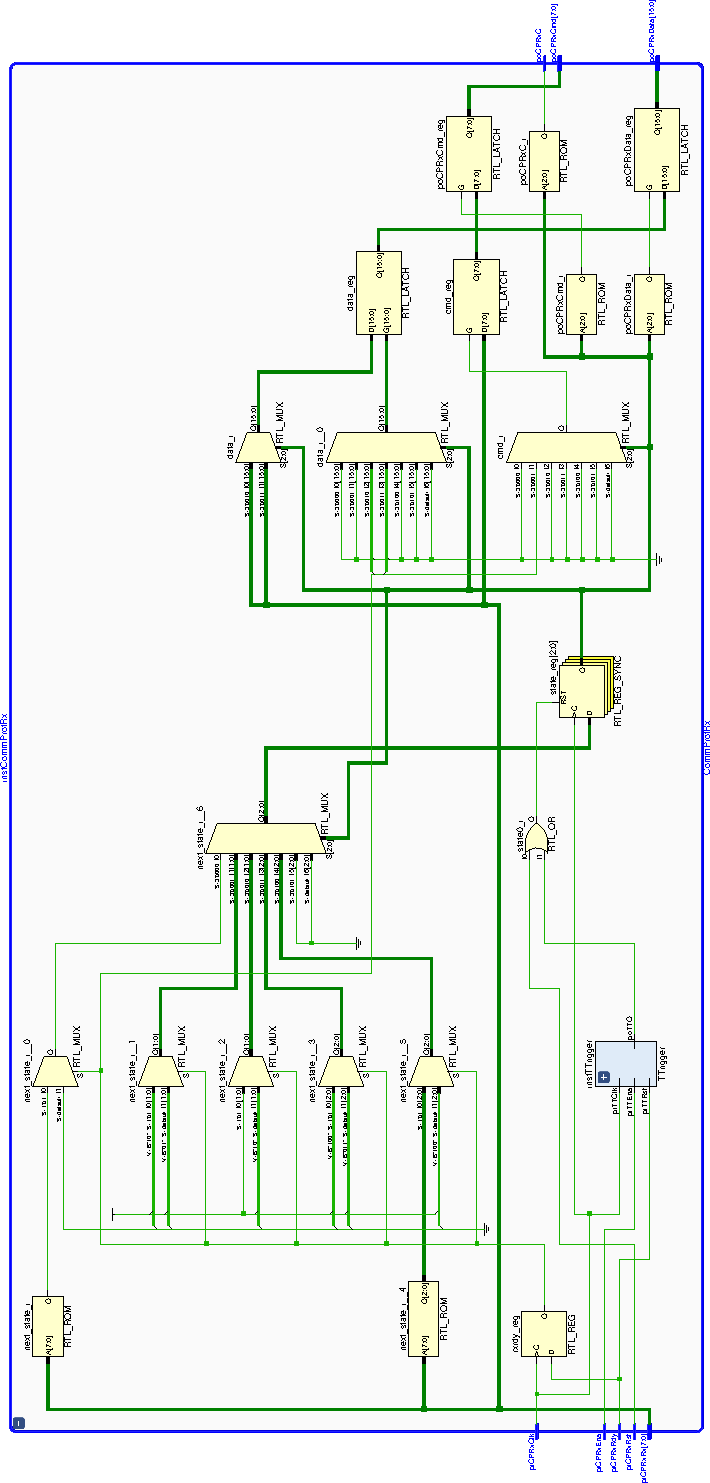
\includegraphics[angle=270, width=0.95\textwidth]{CommProtRx-crop}
    \caption{Esquemático del módulo \textbf{CommProtRx}}
\end{figure}

Si el periodo entre la recepción de los bytes desde el modulo RX en algún momento supera los 100ms, se dispara el trigger de timeout y la detección del paquete de protocolo se reinicia.

\subsection{DecodeCmd}
Cuando se recibe un comando en CommProtRx el mismo se interpreta en este modulo, si el comando corresponde a un comando válido, se interpreta los datos de entrada y se modifica el estado de los motores o sensores si corresponde.

El módulo incorpora un contador de modulo que controla y ajusta la velocidad de los motores cada 10ms según el valor de los sensores, para cuando estos operan en modo automático. Este control periódico no es necesario por tratarse de un control con un valor de corrección fijo, que es aún mas básico de que un control proporcional, pero si lo seria si se incorpora un control PD o PID.

\begin{figure}[H]
    \centering
    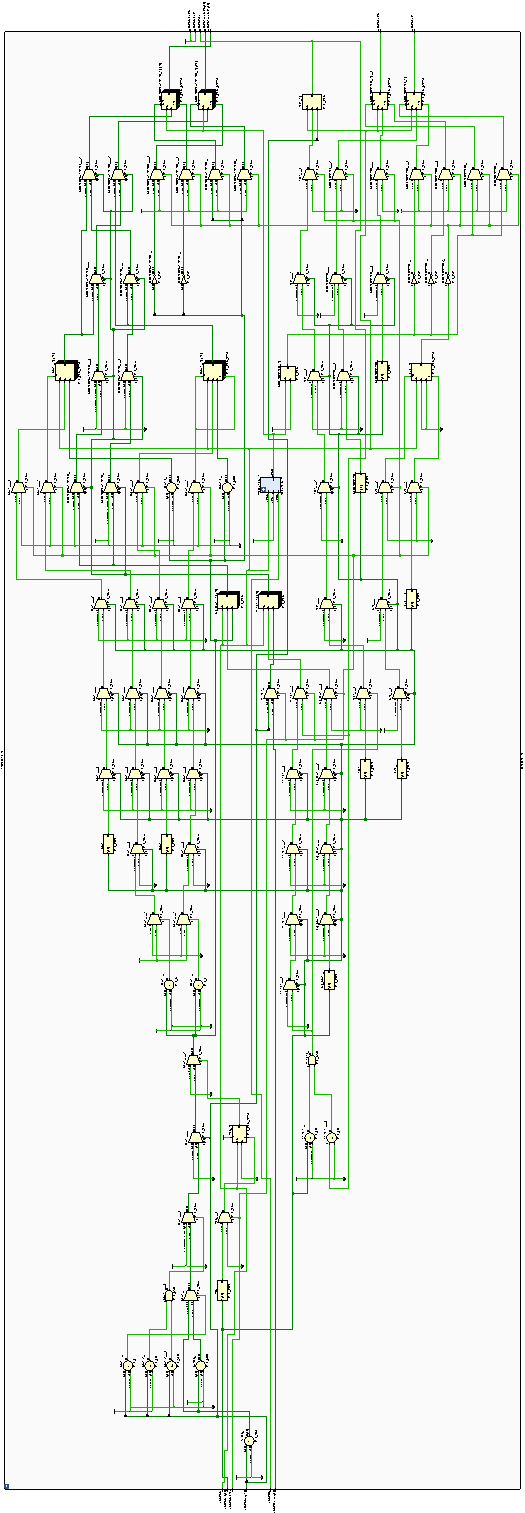
\includegraphics[angle=270, width=\textwidth]{decode-cmd-crop}
    \caption{Esquemático del módulo \textbf{DecodeCmd}}
\end{figure}

\subsection{HBridgeCtrl}
Al recibir un pulso en el puerto set, el módulo registra las entradas duty cycle y dirección de giro, y mediante un modulo PwmGen genera una salida Pwm  y setea las salidas de dirección. El diseño posee dos módulos HBridgeCtrl, uno para cada motor.

\begin{figure}[H]
    \centering
    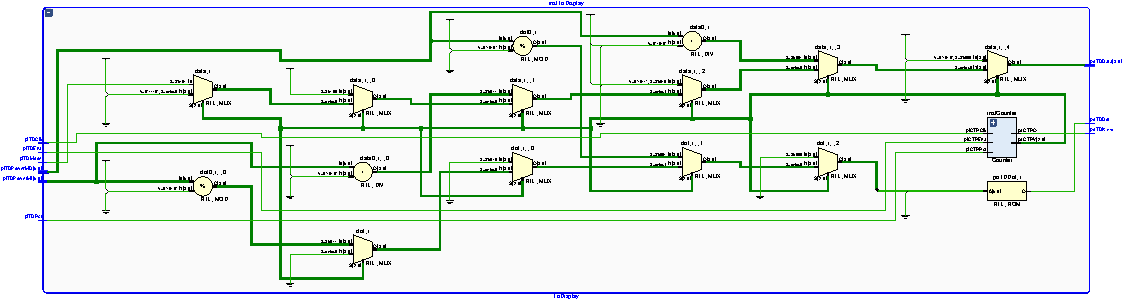
\includegraphics[width=\textwidth]{to-display-crop}
    \caption{Esquemático del módulo \textbf{HBridgeCtrl}}
\end{figure}

Adicionalmente, este modulo tiene como salida los valores actuales de duty cycle y direccion, para que sean tomados por el modulo ToDisplay

\subsection{ToDisplay}

Tiene como entradas la dirección y duty cycle de cada motor además del modo de operación actual del auto, y mediante un modulo Counter muestra de manera cíclica durante 1 segundo los valores de salida, del siguiente modo y en el siguiente orden:
\begin{enumerate}
\footnotesize
\item La letra \textbf{a}
\item La decena de la velocidad del motor Derecho, por ejemplo para un 85\% muestra el numero 8
\item El punto decimal, para el caso donde el duty cycle es 5\% en exceso a la decena, para 85\% se muestra el punto, para 80\% no se muestra.
\item La letra \textbf{b}
\item El duty cilce del motor Izquierdo, del mismo modo que para el motor Derecho
\item La letra \textbf{F}
\item El modo de control, \textbf{0} para modo \textbf{desde PC} o 1 para modo \textbf{desde sensores}.
\end{enumerate}

La salida es un valor hexadecimal de 4 bits mas una salida para el punto.
\begin{figure}[H]
    \centering
    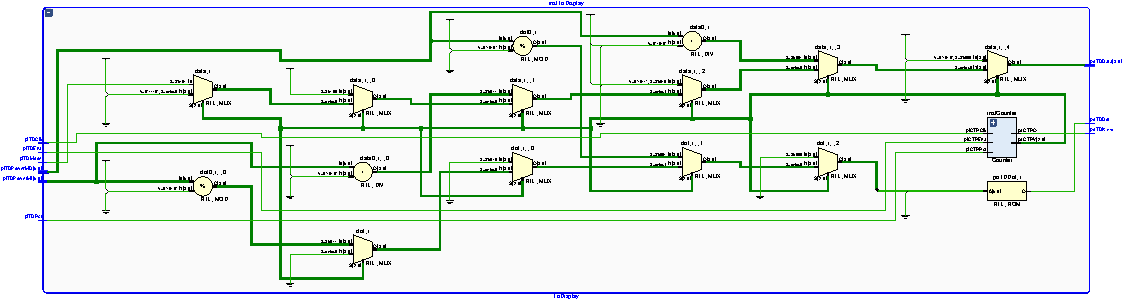
\includegraphics[width=\textwidth]{to-display-crop}
    \caption{Esquemático del módulo \textbf{ToDisplay}}
\end{figure}

\subsection{Módulos auxiliares}
Son módulos de índole mas genérica, muchos de ellos son variaciones de contadores de modulo ajustados al propósito que se busca.

Esto es porque, a diferencia de un programa destinado a generar código ejecutable donde la modularización mediante funciones permite reducir notablemente el tamaño del programa en memoria, en hardware no se posee esta ventaja, un mismo modulo que se instancia dos veces da como resultado dos implementaciones independientes dentro del FPGA. Por esto puede resultar conveniente que cada diseño se ajuste exactamente a lo necesario.


\subsubsection{ModuleCounter}
Diseño básico de un contador de módulo. Se tiene como entrada una señal de clock, un contador interno mantiene un valor que se incrementa con cada clock, cuando se alcanza la cantidad configurada por diseño se genera un pulso de salida y reinicia la cuenta.

\begin{figure}[H]
    \centering
    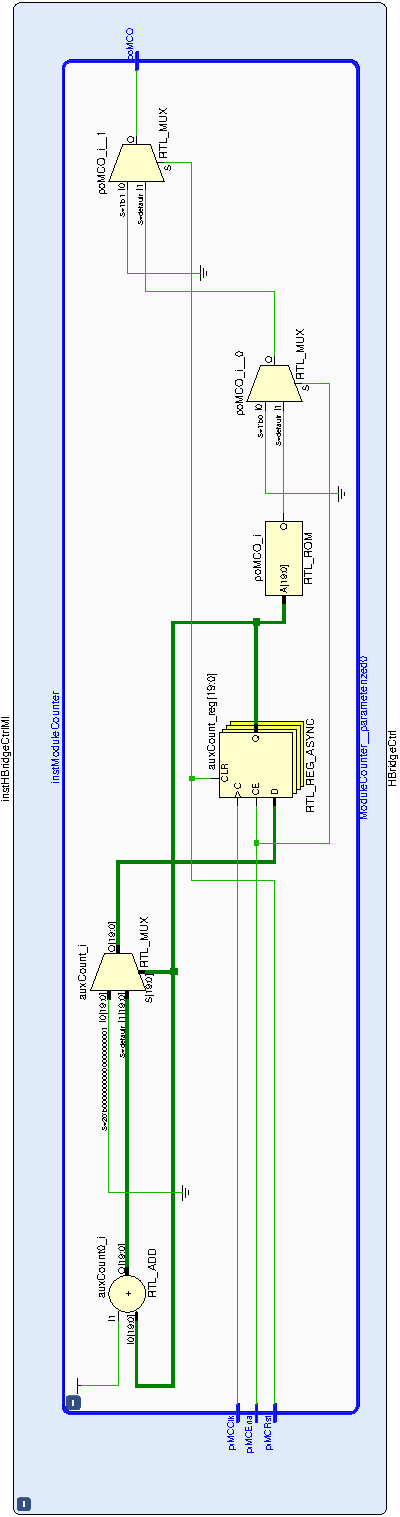
\includegraphics[angle=270, width=\textwidth]{ModCounter-crop}
    \caption{Esquemático del módulo \textbf{ModuleCounter}}
\end{figure}

Este diseño lo utiliza el modulo DecodeCmd para realizar la actualización de la velocidad de los motores segun la lectura de los sensores.

\subsubsection{Counter}
Se trata de un modulo que engloba un contador mas un contador de modulo.
La salida es un bus de N bits que se va incrementando cada vez que el contador de modulo interno alcanza su valor.
\begin{figure}[H]
    \centering
    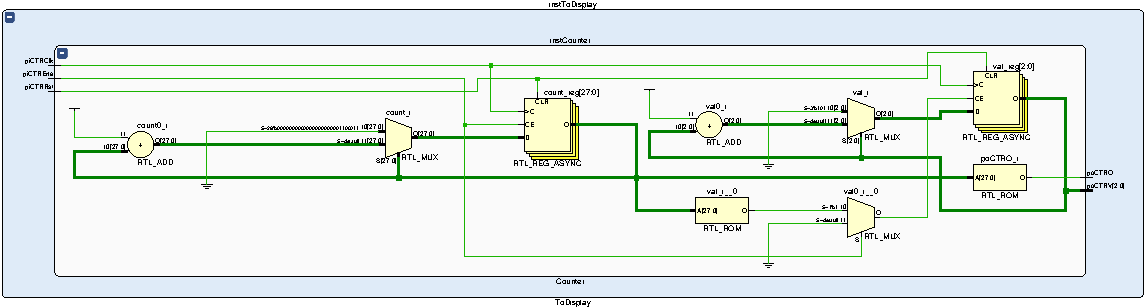
\includegraphics[width=\textwidth]{counter-crop}
    \caption{Esquemático del módulo \textbf{Counter}}
\end{figure}

Es utilizado por el modulo ToDisplay para rotar entre los valores a mostrar en el display de siete segmentos.

\subsubsection{BaudRateGen}
Genera los pulsos de sincronización de baudios para los módulos UaRx y UaTx, se preconfigura con los valores de \textbf{Max} y \textbf{First}, el primer pulso generado tras un reset es de \textbf{First} cantidad de clocks mientras que el resto es de \textbf{Max} cantidad de clocks.

\begin{figure}[H]
    \centering
    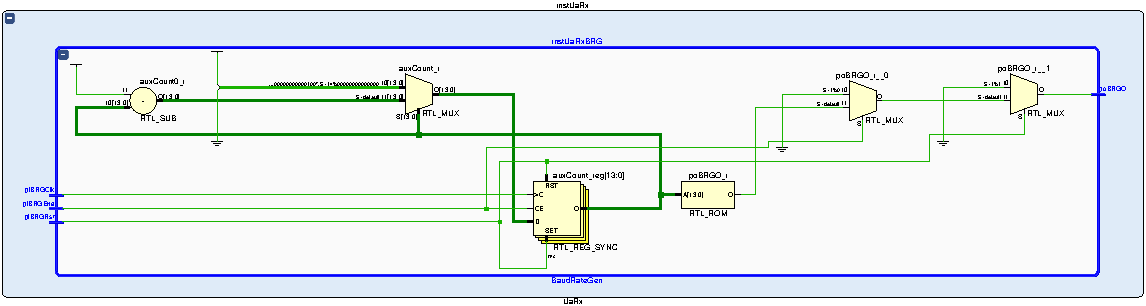
\includegraphics[width=\textwidth]{BaudRateGen-crop}
    \caption{Esquemático del módulo \textbf{BaudRateGen}}
\end{figure}

EL modulo UaTx no requiere que el primer pulso sea de menor duración por lo que su configuración para ese caso es $Max = First$
\subsubsection{TTrigger}
Un contador de modulo, pero donde su salida no es un pulso sino que queda latcheada en alto cuando se alcanza el valor configurado. Se vuelve a low tras un reset y la cuenta se reinicia.

\begin{figure}[H]
    \centering
    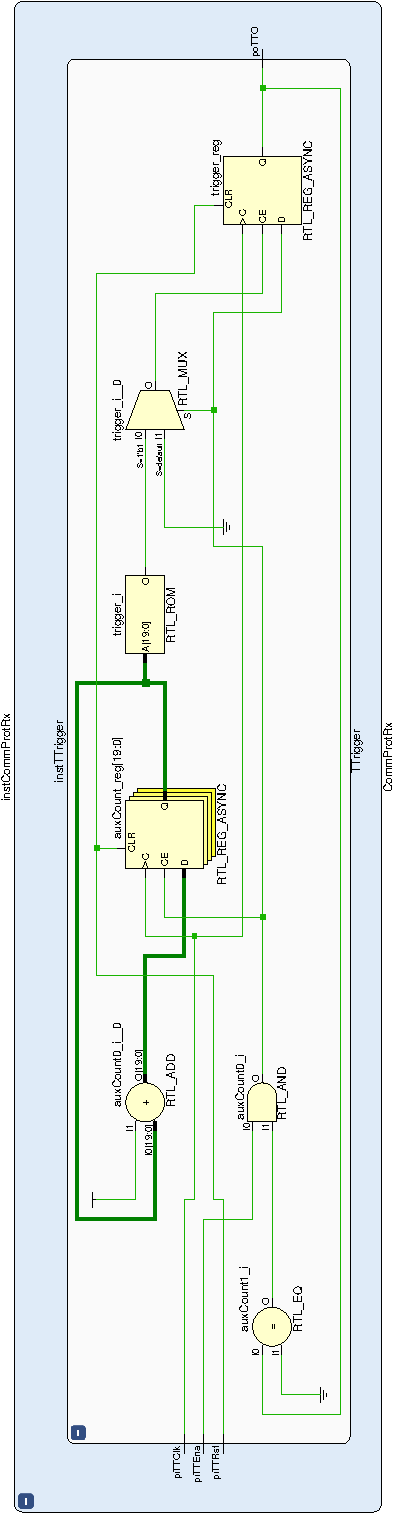
\includegraphics[angle=270, width=\textwidth]{ttrigger-crop}
    \caption{Esquemático del módulo \textbf{TTrigger}}
\end{figure}

Es utilizado por el modulo CommProtRx para detectar timeout.

\subsubsection{PwmGen}
Genera una salida PWM de periodo y resolución variable.
\begin{figure}[H]
    \centering
    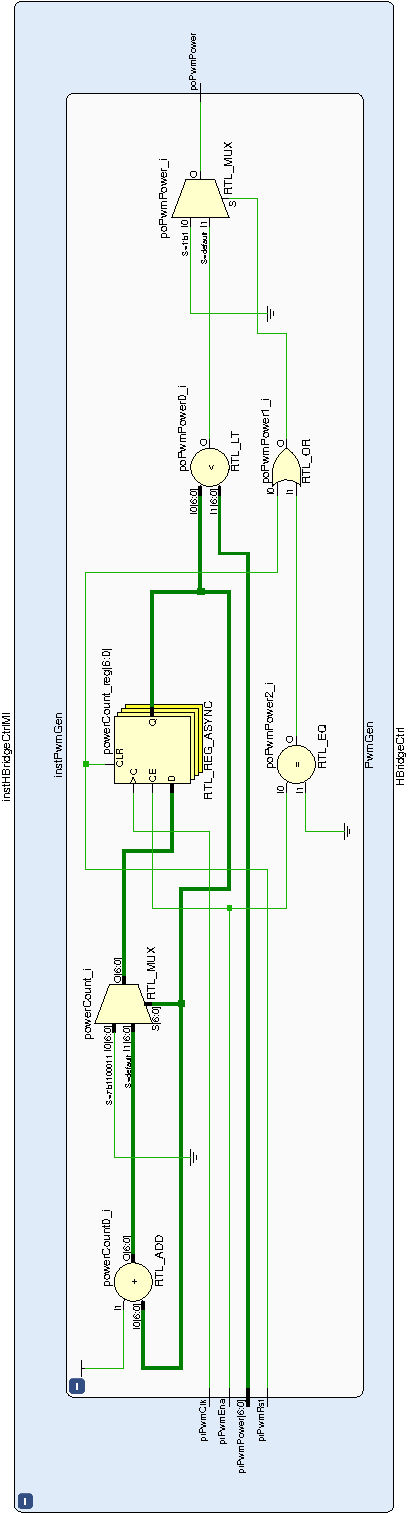
\includegraphics[angle=270, width=\textwidth]{PwmGen-crop}
    \caption{Esquemático del módulo \textbf{PwmGen}}
\end{figure}

\subsubsection{HexToSevSeg}
Decodifica un Hexadecimal de 4 bits en su correspondiente valor de 7 bits para un display de 7 segmentos.
\begin{figure}[H]
    \centering
    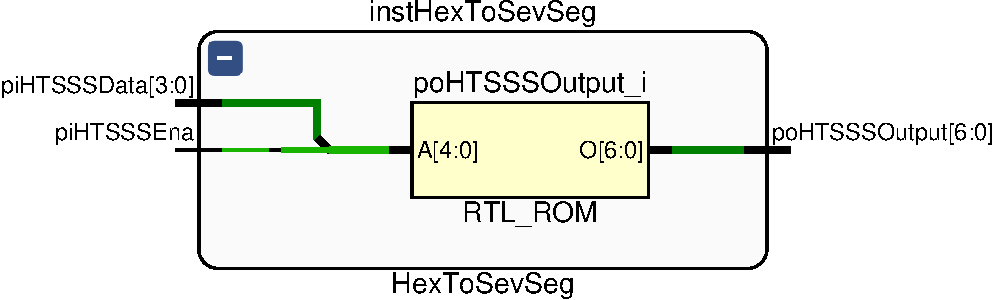
\includegraphics[width=0.6\textwidth]{hex-to-sev-seg-crop}
    \caption{Esquemático del módulo \textbf{HexToSevSeg}}
\end{figure}

\section{Simulación}

Cada modulo se desarrollo con su propio testbench y, adicionalmente, se desarrolló un testbench para la implementación completa, de modo de visualizar el comportamiento global.

\begin{figure}[H]
    \centering
    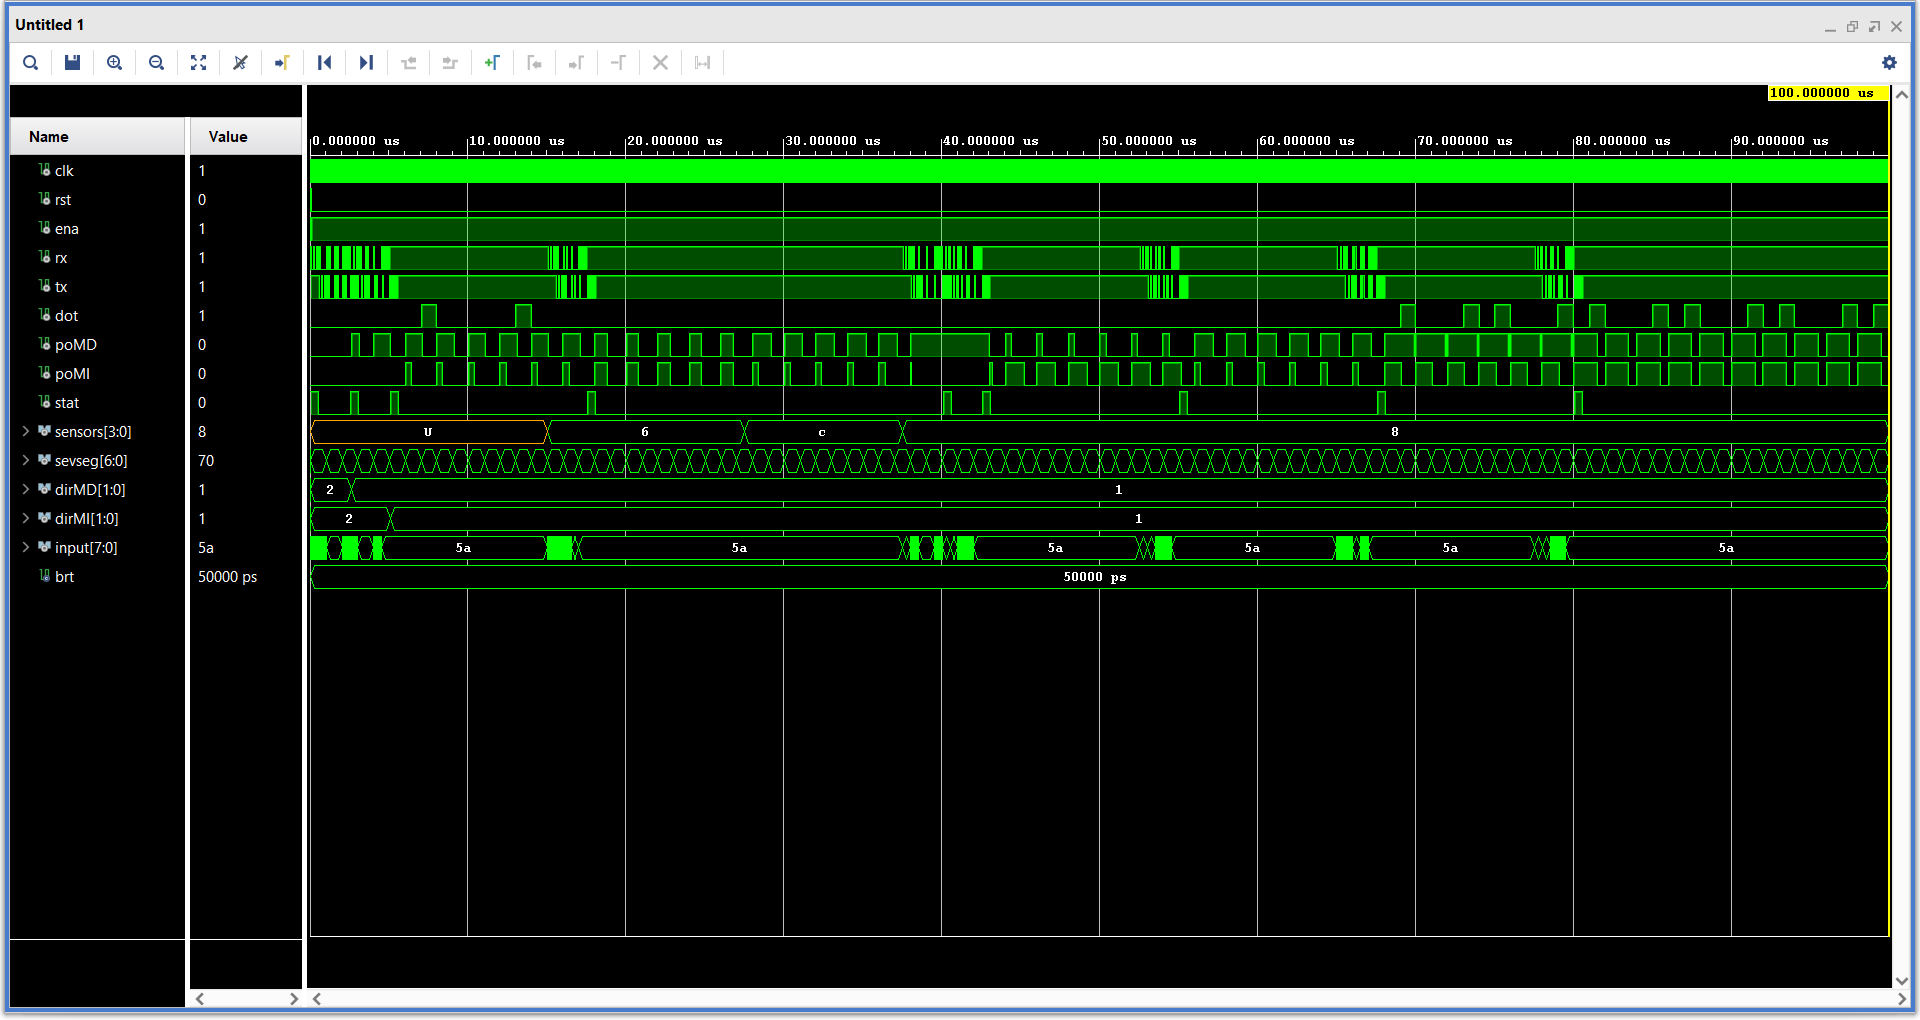
\includegraphics[width=\textwidth]{sim1}
    \caption{Simulación del sistema}
\end{figure}

La simulación consiste en enviar una serie de comandos y ver la respuesta del sistema con un tiempo de espera entre ellos, la respuesta es la esperada. Los comandos son los siguientes:

\begin{enumerate}
\footnotesize
\item Seteo de la velocidad del Motor Derecho a \textbf{55\%} y velocidad Motor izquierdo al \textbf{20\%}.
\item Seteo a modo automático, aplicando velocidad media \textbf{40\%} y sensores físicos con lectura \textbf{0110}
\item Cambio en estado de los sensores a \textbf{1100}, se espera un incremento en \textbf{20\%} del PWM derecho y reducción en \textbf{10\%} del Izquierdo 
\item Cambio en estado de los sensores \textbf{1000}, se espera un \textbf{100\%} en el PWM derecho y \textbf{0\%} en el izquierdo.
\item Cambio a modo de control 1: \textbf{desde PC}, control simulado de sensores a \textbf{0011}.
\item Control simulado de sensores a \textbf{1100}
\item Velocidad media del \textbf{75\%}
\item Control manual de sensores a \textbf{0110}
\end{enumerate}

La siguiente imagen muestra el detalle de la simulación durante la recepción del segundo comando, que hace el seteo a modo automático, aplicando velocidad media \textbf{40\%}.
\\

El modulo UaRx recibe los bytes mediante rs232, el modulo UaTx responde con cada byte recibido. Una vez que el modulo CommProtRx detecta un paquete de protocolo válido dispara el modulo TTrigger que mantiene en alto la salida poMIStat, conectada al led de la placa \textbf{LED0\_R} y se modifica el valor de salida PWM para los dos motores

\begin{figure}[H]
    \centering
    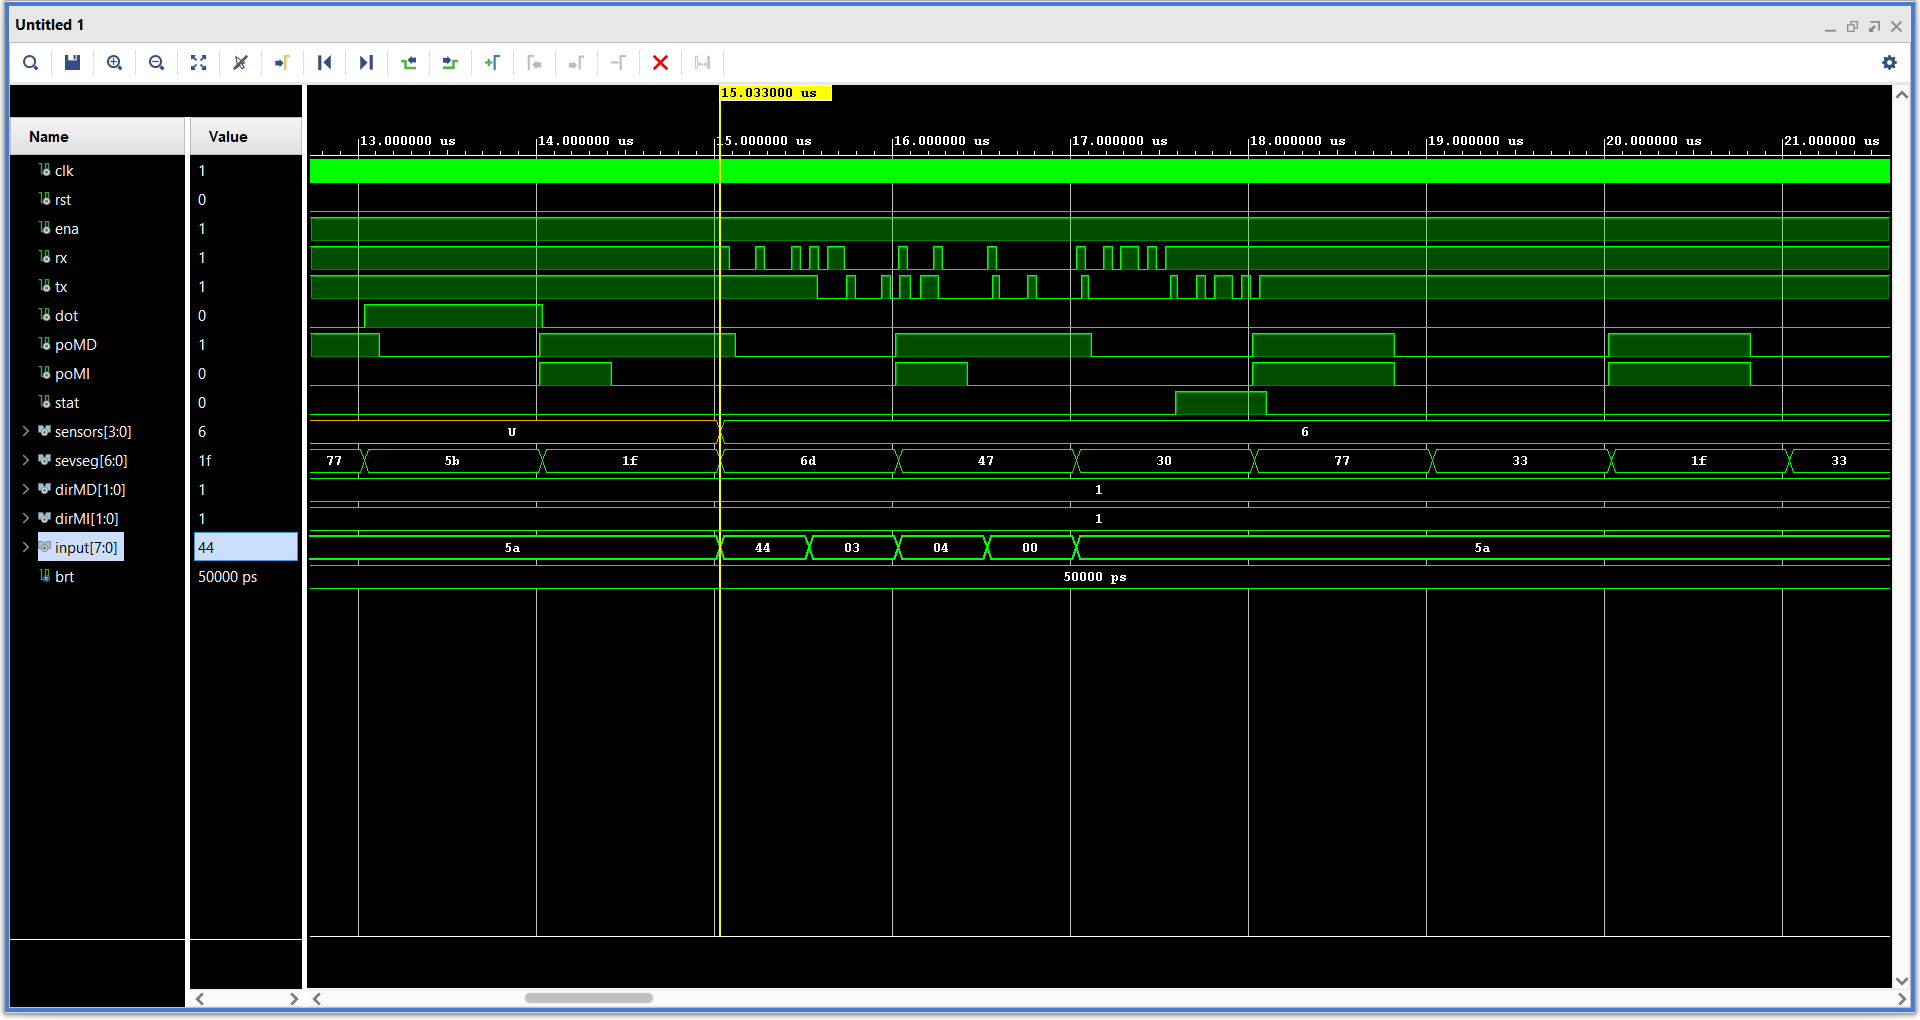
\includegraphics[width=\textwidth]{sim-cmd}
    \caption{Simulación del sistema - Detalle de la recepción de un comando}
\end{figure}

\newpage
\section{Conclusiones}
El desarrollo del auto seguidor de línea en VHDL permitió integrar y aplicar conceptos fundamentales del diseño digital, como el diseño y uso de módulos UART, PWM, maquinas de estado y contadores, que jugaron un papel clave en la generación de señales de control y temporización. Este proyecto consolidó el conocimiento técnico y ofreció una perspectiva práctica sobre cómo los sistemas digitales interactúan con el entorno físico.
\\

Uno de los principales desafíos enfrentados fue la sincronización en el módulo de recepción (RX) del UART en el lado del FPGA, donde se identificaron problemas relacionados con el manejo de señales asíncronas y la correcta alineación temporal de los datos recibidos y el desafío de realizar la depuración.
\\

En conclusión, este proyecto cumplió con los objetivos planteados, superando desafíos técnicos significativos y proporcionando posibles mejoras a futuro, como podría ser la implementación de algoritmos de control PID en lugar de solo un control de valor fijo.

\end{document}
